\documentclass[../thesis.tex]{subfiles}

\begin{document}

\chapter{Implementierung}
\label{chp: implementierung}

Um die Bewertung eines Modells vornehmen zu können, sind einige Bedingungen notwendig. Die experimentellen Daten müssen in einem standardisierten Format zur Verfügung stehen. Die Daten des Modells müssen, sofern das möglich ist, berechnet und anschließend gespeichert werden. Um die Bewertung zu vereinfachen, sollte die Art und Weise, wie die experimentellen Daten und die Daten des Modells gespeichert werden identisch sein. Wenn die experimentellen Daten, sowie die des Modells vorliegen kann der Vergleich und die Bewertung durchgeführt werden. Die Ergebnisse dieses Vergleichs werden, analog zu den Daten, in einem standardisierten Format gespeichert. Als Datenformat bietet sich \texttt{.json} an.

Die Implementierung lässt sich, anhand des beschriebenen Vorgehens, in drei verschiedene Bestandteile aufteilen, welche in den folgenden Abschnitten näher erläutert werden.

\section{Datenbank}

Die Klasse \texttt{database} dient zur Bereitstellung und Speicherung aller benötigten Daten. Diese Daten beinhalten sowohl die der Experimente, als auch die des Modells. Die Klasse Datenbank erzeugt im gleichnamigen Ordner für jedes Gemisch eine eigene Datei, in der alle Daten im \textit{.json} Format abgelegt sind. Der beispielhafte Aufbau einer Gemischdatei ist in \autoref{code: beispielgemisch} dargestellt.

\definecolor{codehighlight}{rgb}{0.95,0.8,0.8}
\lstinputlisting[language=Python, caption=Gemischdatei Beispiel, basicstyle=\fontsize{7}{8}\selectfont\ttfamily
]{./code/gemischbeispiel.json}
\label{code: beispielgemisch}

Der Schlüssel \texttt{BAC} dient der Klassifizierung des Gemisches, wie in \autoref{sec: gemischklassifikation} beschrieben. Das Tabellenblatt auf dem die Daten in der Originaldatei zu finden sind ist als Wert des Schlüssels \texttt{sheet} gespeichert. Analog zum Aufbau der Originaldatei werden unter den weiteren Schlüsseln die Daten der gemessenen Größen gespeichert. Alle Messreihen werden als Liste unter dem jeweiligen Variablennamen gespeichert.

Eine Messreihe ist durch ihre Quelle unter dem Punkt \texttt{reference}, die Parameter der Messung unter dem Punkt \texttt{params}, und die Messdaten unter dem Punkt \texttt{measurements} charakterisiert.

Somit stehen alle experimentellen Daten in computerlesbaren Format zur Verfügung.

\section{Modell}

Die Klasse \texttt{model} dient dazu die Daten des Modells bereitzustellen, damit diese anschließend mit den experimentellen Daten verglichen und bewertet werden können.

Der Ablauf der Berechnung für ein Gemisch ist in \autoref{fig: model_berechnung} gezeigt.

\begin{figure}[htb]
	\centering
	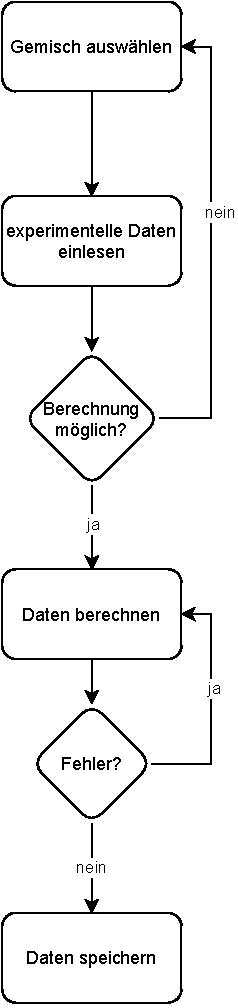
\includegraphics[scale=0.7]{berechnung_model}
	\caption{Ablauf Berechnung Model}
	\label{fig: model_berechnung}
\end{figure}

Für jedes Gemisch werden die folgenden Schritte für jede zu berechnende Größe durchgeführt. Als erster Schritt wird das zu berechnende Gemisch festgelegt. Anschließend werden alle vorhandenen experimentellen Daten aus der entsprechenden \texttt{.json} Datei eingelesen. Die hier eingelesenen Daten bestimmen was das Modell berechnen soll. Es werden alle Größen, die für das Gemisch gefunden wurden nacheinander berechnet. Bevor das Modell aufgerufen wird, wird getestet ob das Modell die Daten für das Gemisch überhaupt berechnen kann. Dieser Test basiert auf den Parametern, die für das Modell vorhanden sind. Ist ein Stoff an dem Gemisch beteiligt für den das Modell keine Parameter, hat kann das Modell keine Ergebnisse berechnen. Dieses Gemisch wird übersprungen.
Kann das Modell die geforderten Daten berechnen wird es aufgerufen und wenn kein Fehler bei der Berechnung auftritt werden die Daten gespeichert. Andernfalls wird versucht den nächsten Datenpunkt zu berechnen. Die Datei mit den Berechnungsergebnissen des Modells hat den gleichen Aufbau, wie die der experimentellen Daten aus Listing \autoref{code: beispielgemisch}

\section{Bewertung}

Die Klasse Bewertung dient dazu den Vergleich der experimentellen und den aus dem Modell berechneten Daten durchzuführen. Als Ergebnis werden die Teilnoten der betrachteten Systeme und Klassen, sowie die Gesamtnote des Modells berechnet.

\subsection{Bewertung Mischungswärmekapazität und Mischungsenthalpie}

Für die Wärmekapazität werden die berechneten Daten mit den experimentellen Daten wie in \autoref{glg: } verglichen. Da für alle experimentellen Datensätze Werte berechnet werden können ist gewährleistet, dass die Anzahl der zur Verfügung stehenden experimentellen Daten mit der Anzahl der aus dem Modell erhaltenen übereinstimmt.

Dies stimmt auch für die Mischungswärmekapazität.

\subsection{Bewertung Phasengleichgewichte}

Für die Bewertung der Phasengleichgewichte müssen die Daten des Modells und die experimentellen Daten zusammengeführt werden. Das Modell berechnet typischerweise eine weit aus größere Anzahl an Datenpunkt als im experimentellen Datensatz vorliegen.  Um die experimentellen Datenpunkte in denen des Modells zu finden wird zuerst der korrekte Datensatz gesucht. Im Falle eines isobaren Phasengleichgewichts ist dies der Datensatz ,welcher als Parameter den gleichen Druck $p$ enthält. Für ein isothermes Phasengleichgewicht wird anstatt des Drucks $p$ nach der identischen Temperatur $T$ als Parameter gesucht. Kann der Datensatz nicht gefunden werden, wird mit dem nächsten fortgefahren.

Ist der Datensatz vorhanden wird in Berechnungsergebnissen nach dem Punkt gesucht der die kleinste Abweichung vom zweiten Parameter hat. Für ein isothermes Phasengleichgewicht ist dies der Druck $p$ und für ein isobares die Temperatur $T$. Liegt der gefundene Datenpunkt außerhalb des Modells wird der Datenpunkt verworfen und mit dem nächsten fortgefahren. Ein experimenteller Datenpunkt liegt außerhalb des Modells, wenn die Größe des zweiten Parameters kleiner als der minimale oder größer als der maximale vom Modell berechnete Wert ist. Das in \autoref{fig: phase_eq_datenausschluss} isotherme Phasengleichgewicht für das binäre Stoffgemisch aus Dichloromethan und Kohlenstoffdisulfid ist ein Beispiel für den Fall, dass alle experimentellen Punkte außerhalb des Modells liegen. 

\begin{figure}[htb]
	\centering
	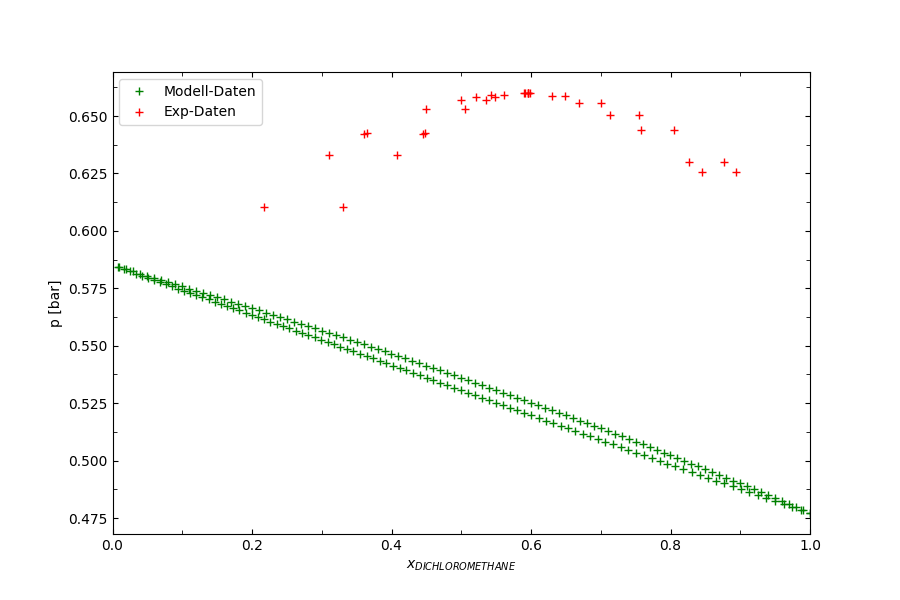
\includegraphics[scale=0.6]{DICHLOROMETHANE_CARBON DISULFIDE_isotherm_298.15_}
	\caption{Isothermes Phasengleichgewicht bei $ 298.15 K$ für das Stoffgemisch Dichlormethan|Kohlenstoffdisulfid}
	\label{fig: phase_eq_datenausschluss}
\end{figure}

Anschließend werden die entsprechenden Molenbrüche der Flüssigkeit $x$ und der Gasphase $y$ zwischengespeichert.

Sind alle Datensätze durchsucht worden, werden die zwischengespeicherten Molenbrüche miteinander verglichen und bewertetet.

\subsection{Bewertung azetroper Punkt}

Für die Bewertung des azeotropen Punkts werden die Modelldaten dieses Punktes benötigt. Da es keine direkte Berechnungsmethode in \texttt{TREND} für diese Größe gibt wird dieser aus den berechneten Phasengleichgewichtsdaten extrahiert. Die Methode durchsucht nur diejenigen Stoffgemische, bei denen in den experimentellen Phasengleichgewichten azeotrope Punkte vermerkt wurden. Da der azeotrope Druck als Bewertungsgröße definiert ist, werden nur isotherme Phasengleichgewicht betrachtet da nur hier der Druck berechnet und verändert wird. Um den azeotropen Punkt zu finden wird nach dem Maximum bzw. Minimum des Drucks in den Daten gesucht und die zugehörigen Molenbrüche gespeichert. Azeotrope Gemische können als Druckmaximumazetrope wie in \autoref{fig: durckmaximumazeotrop} dargestellt oder als Druckminimumazeotrope wie in \autoref{fig: druckminimumazeotrop} zu sehen auftreten. In beiden Fällen wird die Abweichung des vom Modell berechneten Drucks und die Abweichung der vom Modell berechneten Zusammensetzung $x$ von den experimentellen Werten bewertet. Eine separate Bewertung der Zusammensetzung der Dampfphase $y$ ist nicht notwendig, da diese am azeotropen Punkt gleich der der Flüssigphase ist.  

\begin{figure}[htb]
	\centering
	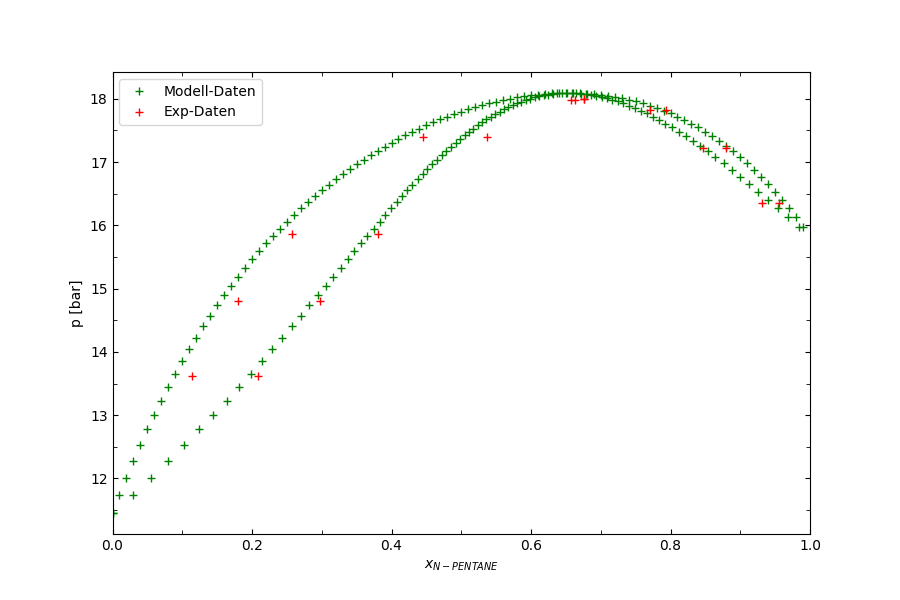
\includegraphics[scale=0.5]{ACETONE_N-PENTANE_isotherm_422.6_}
	\caption{Isothermes Phasengleichgewicht bei $ 422.6 K$ für das Stoffgemisch Azeton|n-Pentan}
	\label{fig: durckmaximumazeotrop}
\end{figure}

\begin{figure}[htb]
	\centering
	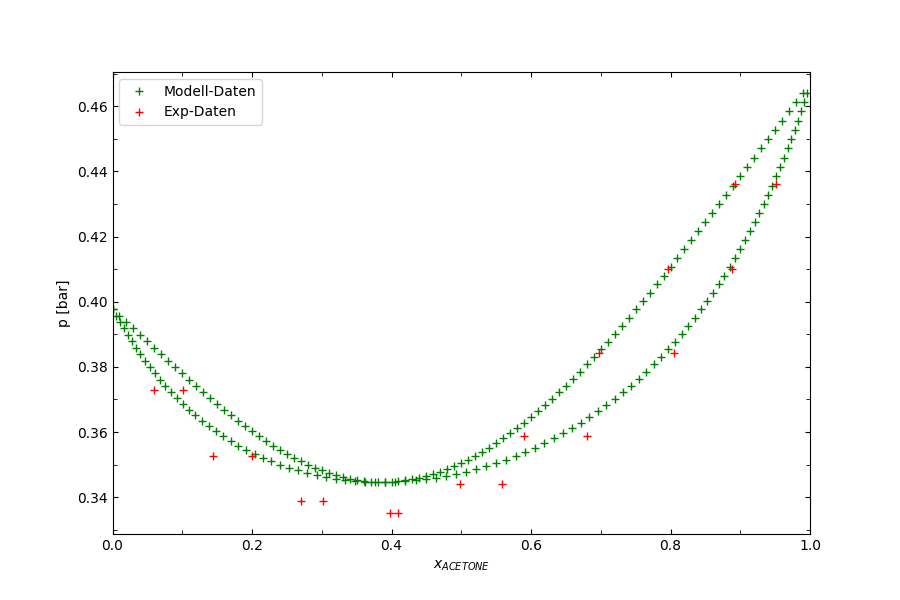
\includegraphics[scale=0.5]{CHLOROFORM_ACETONE_isotherm_308.15_}
	\caption{Isothermes Phasengleichgewicht bei $ 308.15 K$ für das Stoffgemisch Chloroform|Azeton}
	\label{fig: druckminimumazeotrop}
\end{figure}

\subsection{Bewertung weiterer Zustandsgrößen}

Die weiteren Zustandsgrößen des Gemisches wie die des kritischen Punkts $ p_{\mathrm{c}}$ und $ x_{\mathrm{c}}$, sowie die 3-Phasen Zustandsgrößen $p_{\mathrm{LLV}}$ und $z_{\mathrm{LLV}}$ können vom Modell bisher nicht berechnet werden, da die nötigen Routinen bisher nicht stabil genug funktionieren oder noch nicht implementiert wurden.

Aufgrund der fehlen Daten des Modells können für diese Größen bisher keine Noten berechnet werden, sodass diese in der Bewertung des thermodynamischen Modells bisher nicht berücksichtigt werden.

\end{document}
